% =====================================================================
%  c29 —— 原文印刷页 243--244（PDF 第 244--245 页）
%  含：L.3 末尾（图 40 与有向配边环的结构定理）、L.4 其他配边范畴、
%      M. 课程笔记中的若干来源、致谢（Acknowledgements）
%  编号公式：L.7、L.8；插图：Fig. 40。
%  注：印刷页 244 下半页起为 References（[1]--[72]），按分工由 chunks/c-refs.tex
%      处理，本片段到「References」标题之前为止，不转写任何文献条目。
%  全部内容逐页对照 150 dpi 页面图像（p244.png、p245.png）核校。
% =====================================================================

\begin{figure}[htbp]
  \centering
  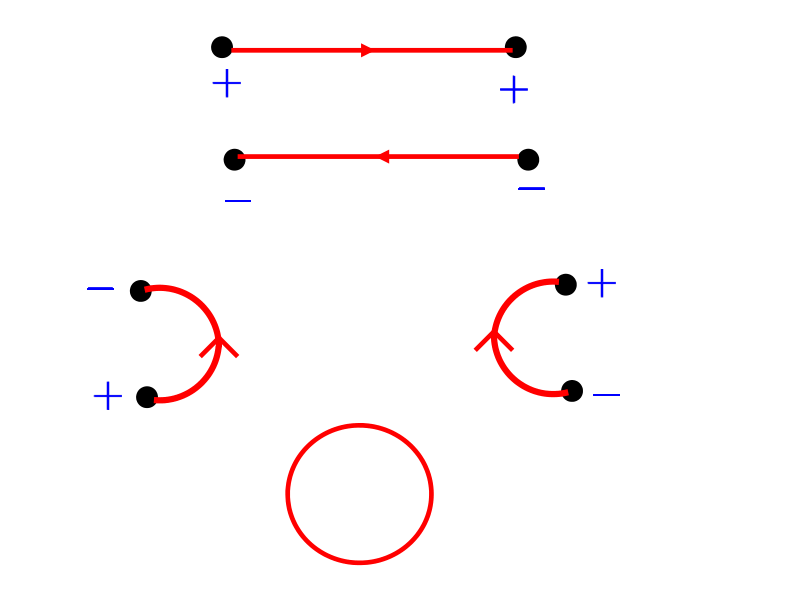
\includegraphics[width=0.55\textwidth]{figures/fig40.png}
  \caption{有向配边范畴中的五个连通配边。入边界在左，出边界在右。（原文 Fig.~40，第 243 页）}
  \label{fig:40}
\end{figure}

关于有向配边环 $\Omega_*^{SO}$ 的主要因子，总结如下。（见 Milnor 与 Stasheff。Freed 的讲义中在定理 2.24 附近还给出了若干进一步的文献。）\footnote{若我们讲到特征类那一章，就会证明其中一些结果。}

% 转写说明：原文此处只印有粗体的「Theorem」，并无编号；此处沿用主文件预定义的
% theorem 环境（与 c23 中同类情形一致），编号由 LaTeX 自动生成。

\begin{theorem}
\normalfont % 原文定理正文为直立体；中文无真正的斜体，故置正体（数学模式不受影响）
\begin{enumerate}
  \item $\Omega_*^{SO}$ 中所有挠元（torsion element）的阶都是二。
  \item $\Omega_*^{SO}/\,\mathrm{torsion}$ 是一个环，它在每个次数 $4k$（$k\ge 1$）上恰有一个生成元。
  \item 存在同构
  \begin{equation}
    \Omega_*^{SO}\otimes\mathbb{Q} \cong \mathbb{Q}[y_4,y_8,\cdots]
    \tag{L.7}
    \label{eq:L.7}
  \end{equation}
  在此同构下，$y_{4k}$ 对应于 $\mathbb{CP}^{2k}$ 的有向配边类。
  \item $Y$ 的切丛有特征类，即 Stiefel-Whitney 类 $w_i(Y)\in H^i(Y;\mathbb{Z}_2)$ 与 Pontryagin 类 $p_i(Y)\in H^{4i}(Y;\mathbb{Z})$（后者依赖于 $Y$ 的定向），使得 $Y_1$ 与 $Y_2$ 配边当且仅当所有 Stiefel-Whitney 数与 Pontryagin 数都相同。我们上文已定义了 Stiefel-Whitney 类，而 Pontryagin 数同样是如下这一族数
  \begin{equation}
    \langle p_{i_1}(Y)\cup\cdots\cup p_{i_k}(Y),[Y]\rangle \in \mathbb{Z}
    \tag{L.8}
    \label{eq:L.8}
  \end{equation}
\end{enumerate}
\end{theorem}

% [Tutor Note: 作者所说的「主要因子」(main factors) 指环 $\Omega_*^{SO}$ 的乘性生成元
% （即环论意义下的「素因子」），不是「主要因素」；译作「主要因子」只为与原文用词对应。
% 第 2 条与第 3 条须合读：第 2 条给出无挠部分在每个次数 $4k$ 上一个生成元，第 3 条则说明
% 张量 $\mathbb{Q}$ 后挠元消失（正是第 1 条「阶为二」的直接后果：阶为二的元素在
% $\mathbb{Q}$-系数下变成零），剩下的多项式环由 $y_{4k}\leftrightarrow[\mathbb{CP}^{2k}]$
% 生成。核对次数时注意 $\mathbb{CP}^{2k}$ 的\emph{实}维数是 $4k$，所以生成元次数为
% $4,8,12,\dots$ 即 $4k$，不是 $2k$；若误记为 $2k$，(L.7) 右端的下标就要全部改成
% $y_2,y_4,\dots$，而这与 (L.8) 中 Pontryagin 类所在次数 $4i$ 无法配对。]

% [Tutor Note: 定理第 4 条原文印作「such that $Y_1$ and $Y_2$ and bordant iff …」，
% 第二个 and 显然是 are 的笔误（应为「$Y_1$ and $Y_2$ are bordant iff …」），中文无法保留
% 这处拼写错误，故按文意译作「$Y_1$ 与 $Y_2$ 配边当且仅当……」。读这条判据时还须注意两件事：
% 其一，「所有 Stiefel-Whitney 数与 Pontryagin 数都相同」里的「所有」是指对一切可行多重指标
% $i_1\le\cdots\le i_k$ 取遍，而不是只取一个数；其二，(L.8) 的配对要求 $\dim Y=4(i_1+\cdots+i_k)$，
% 故奇数维流形的 Pontryagin 数全为零，那条判据在奇数维就退化为只看 Stiefel-Whitney 数——
% 这是 Thom 配边定理的标准形式，作者在此只是复述，未给证明（证明要用到 Thom 谱与
% Serre 关于稳定同伦群有限性的结果）。]

\subsection{其他配边范畴} % 原文: L.4 Other Bordism Categories

% 转写说明：原文此行写作「We can go on an consider other forms of bordism:」，
% 其中「an」应为「and」（笔误），译文按文意译出，未保留该拼写错误。

我们还可以接着考虑其他形式的配边：
\begin{enumerate}
  \item 标架配边（framed bordism）。（通过 Pontryagin-Thom 构造，它与球面的稳定同伦密切相关。）
  \item Spin 配边与 Pin$^{\pm}$ 配边。
  \item Riemann 配边（Riemannian bordism）。
\end{enumerate}

相应地，配边范畴也有各种推广。一般地，若我们计入某种结构 $\mathcal{S}$，就把配边范畴记作 $\mathrm{Bord}^{\mathcal{S}}_{\langle d-1,d\rangle}$；这里约定的意思是，配边之间用保持结构 $\mathcal{S}$ 的同胚来等同。于是，有向配边范畴记作 $\mathrm{Bord}^{SO}_{\langle d-1,d\rangle}$（因为切丛的结构群分别是 $SO(d-1)$ 与 $SO(d)$）。类似地我们可以定义 Riemann 配边范畴 $\mathrm{Bord}^{\mathrm{Riem}}_{\langle d-1,d\rangle}$，如此等等。

% [Tutor Note: 记号里上标与下标分工不同，最易写反：上标 $\mathcal{S}$ 是「所附加的结构」
% （定向、Spin、标架、Riemann 度规……），下标 $\langle d-1,d\rangle$ 是「维度档」——对象是
% $(d-1)$ 维闭流形、态射是 $d$ 维配边，与第 5 章的 $\mathrm{Bord}^{S}_{\langle d-1,d\rangle}$
% 完全同一套约定；这里用的是尖括号 $\langle\cdot,\cdot\rangle$，不要写成圆括号。
% 另一处易错点是括号里的结构群：$d$ 维配边的切丛结构群是 $SO(d)$，而其 $(d-1)$ 维边界上
% 因为有指向外（或内）的法向，结构群约化为 $SO(d-1)$，所以原文才说「分别是 $SO(d-1)$ 与
% $SO(d)$」；若在边界上也写 $SO(d)$，边界就带上了法向的冗余信息，配边的粘接不会自洽。
% 术语上 bordism 与 cobordism 在中译里都作「配边」，故本片段统一用「配边」，不加区分。]

\section{课程笔记中的若干来源} % 原文: M. Some Sources From Course Notes

\begin{keytakeaways}
  \item 本节不是论证，而是一份按主题分组的「素材出处」清单：作者把自己历年课程笔记中
    与正文各章配套的部分逐条列出，供读者按主题回溯原始材料。
  \item theta 函数与 Heisenberg 代数的材料见 GMP7-06 第 6 节与
    GMP-Ch8-AssociatedBundles-2010 第 11 节；这正是附录 D、E 中模变换律与环面上全纯线丛
    那套内容的上游笔记。
  \item 第 $k$ 级 theta 函数的\emph{不变范数}与第一 Chern 类见 GMP9-06 第 3.3 节——它对应
    正文中用 theta 函数构造预量子线丛的 Hermitian 结构那一步。
  \item 群上同调与 Dijkgraaf-Witten 理论见 GRP-THEORY-Lect1；拓扑场论与范畴见 GMP 2015。
    这两条分别接续正文关于有限群规范理论与扩展拓扑场论／张量范畴的讨论。
  \item 这些编号（GMP7-06、GMP9-06、GMP-Ch8-AssociatedBundles-2010、GRP-THEORY-Lect1、
    GMP 2015）是作者个人课程笔记的内部编号，不是正式发表的文献条目，因此与下文参考文献表
    互补而不重复。
\end{keytakeaways}

关于 theta 函数与 Heisenberg 代数的材料：
\begin{itemize}[label={},leftmargin=2.6em,itemsep=2pt,topsep=2pt]
  \item GMP7-06, section 6
  \item GMP-Ch8-AssociatedBundles-2010, section 11.
\end{itemize}

第 $k$ 级 theta 函数的不变范数（invariant norm）、第一 Chern 类：GMP9-06, section 3.3.

还有群上同调。一些 Dijkgraaf-Witten 理论。GRP-THEORY-Lect1

拓扑场论与范畴：GMP 2015.

% [Tutor Note: 这一节的行文是笔记索引而非普通段落，其中的「GMP7-06」「GMP-Ch8-
% AssociatedBundles-2010」「GMP9-06」「GRP-THEORY-Lect1」「GMP 2015」都是作者课程笔记的
% 文件名式编号，「section 6」「section 11」「section 3.3」是这些笔记内部的节号。译文照原样
% 保留这些拉丁字符串、未译成「第 6 节」，因为一旦译出就无法再与笔记原件对应；缩进的两行
% 是被「关于 theta 函数与 Heisenberg 代数的材料：」统领的子项，故用无标号列表复刻其缩进，
% 其余各行原文即为顶格，故仍作独立段落。原文各行的句末标点本就不统一（有的有句点、有的
% 没有），译文一仍其旧。]

\subsection*{致谢} % 原文: Acknowledgements

GM 谨向 2019 年 TASI 暑期学校的组织者致谢，感谢他们邀请他作报告。

GM 感谢 Daniel Brennan、Anindya Dey、Roman Geiko、Ahsan Khan、Tom Mainiero、Nati Seiberg 与 Xinyu Zhang 对草稿提出的有益意见。他也感谢 TASI 的学生们提出的许多好问题与评论。特别是 Geoff Penington 与 Babak Vadeqan，他们指出了笔记中的不确切之处。

GM 的工作受 DOE 支持，资助号 DE-FG02-96ER40959。
